\chapter{Blockchain Scalability}
The \textbf{Blockchain trilemma} states that blockchain systems can only achieve two of the following three properties: decentralization, security, and scalability. This is because the three properties are in conflict with each other, and was initially stated by Vitalik Buterin.

\begin{figure}[htbp]
   \centering
   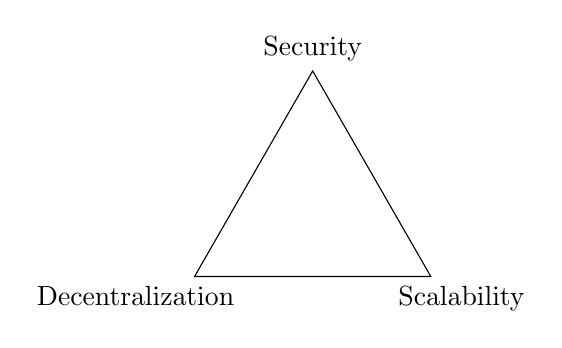
\begin{tikzpicture}[scale=3]
      \draw (0,0) -- (1,0) -- (0.5,0.87) -- cycle;
      \node at (1.13,0) [below] {Scalability};
      \node at (0.5,0.87) [above] {Security};
      \node at (-0.25,0) [below] {Decentralization};
      % \node at (0.5,0.4) {Blockchain Trilemma};
  \end{tikzpicture}
  \caption{Blockchain Trilemma}
   \label{fig:blockchain_trilemma}
\end{figure}

\section{``On-chain'' Scalability}
\textbf{On-chain} scalability refers to the ability of a blockchain to handle a large number of transactions per second. The Bitcoin network can handle 7 transactions per second, while the Ethereum network can handle 15 transactions per second. This is a very low number compared to traditional payment systems like Visa, that can handle 24,000 transactions per second.

On-chain scalability solutions ---each one has pros and cons--- include:
\begin{itemize}
   \item Increase block size
   \item Increase block frequency
   \item Cross-chains and side-chains 
   \item Use alternative consensus algorithms (e.g. \textit{Proof of Stake})
\end{itemize}

\section{``Off-chain'' Scalability}
The key idea for \textbf{off-chain} scalability is to move transactions off the main blockchain, and to settle them on the main blockchain only when necessary. This way, the main blockchain is not overloaded with transactions, and only used as ``arbiter'' when necessary.

Off-chain transactions are like promissory notes, where the parties involved in the transaction exchange IOUs, and settle them on the main blockchain only later on.
The security of such transactions is almost the same of the main chain, but allow for high-volume of instant, trustless, micropayments.

Bitcoin Lightning Network is an example of off-chain scalability solution. It is a second layer protocol that operates on top of the Bitcoin blockchain, and allows for instant, low-fee, micropayments.
Currently the Lightning Network can handle 10,000 transactions per second, and it is growing.

\section{MultiSignature Transactions}
MultiSignature transactions are a way to increase the security of a transaction, by requiring the signature of multiple parties to spend the funds. This can be used to increase the security of off-chain transactions, by requiring the signature of a third party to settle the transaction on the main chain.

They are implemented through the CHECKMULTISIG script, that requires the signature of multiple parties to spend the funds.

Practical MultiSignature use cases are:
\begin{itemize}
   \item 1-of-n: a transaction requires the signature of only one party to spend the funds.
   \item 2-of-2: a transaction requires the signature of both parties to spend the funds.
   \item 2-of-3: a transaction requires the signature of two parties to spend the funds.
   \note{Commonly used for \textit{escrow contracts}}
\end{itemize}

\subsection{Escrow contracts}
An \textbf{escrow\footnote{``Escrow'' means ``deposito in garanzia'' in italian} contract} is a contract where a third party holds the funds until the conditions of the contract are met. The third party is responsible for releasing the funds to the correct party, and can be used to increase the security of a transaction.

Alice wants to buy a product from Bob, but she does not trust Bob. They can use an escrow contract to secure the transaction, by involving the third ---trusted--- party Judy:
\begin{enumerate}
   \item Alice creates a 2-of-3 MultiSignature transaction, where the funds are locked in the escrow contract.
   \item Coins are held in escrow by Alice, Bob and Judy. Any two of them can redeem the funds and specify the receiver of the bitcoins
\end{enumerate}
In case there are no disputes, Alice and Bob can redeem the funds together. If there is a dispute, Judy can decide who ``cheated'' and who gets the funds.\\
In either case, two transactions are needed, one from Alice to the escrow, and another one to either Bob or back to Alice.